\documentclass[11pt,class=report,crop=false]{standalone}
\usepackage[screen]{../python}

% \usepackage{bbding}

\begin{document}
 
%====================================================================
\chapitre{Convolution avec Python}
%====================================================================

\insertvideo{gWoHWXGkdxs}{partie 13. Convolution avec Python}


\objectifs{\Python{} permet de calculer facilement les produits de convolution.} 



\index{convolution!avec Python@avec \Python}

%%%%%%%%%%%%%%%%%%%%%%%%%%%%%%%%%%%%%%%%%%%%%%%%%%%%%%%%%%%%%%%%%%%%%
\section{Convolution et matrices}

%--------------------------------------------------------------------
\subsection{Convolution}

Le module \ci{scipy} fournit une fonction \ci{convolve2d()} qui calcule le produit de convolution $A \conv M$ de deux tableaux \numpy{}.

\begin{lstlisting}
import numpy as np
from scipy import signal

A = np.array([[2,1,3,0],[1,1,0,5],[3,3,1,0],[2,0,0,2]])
M = np.array([[1,0,2],[2,1,0],[1,0,3]])

B = signal.convolve2d(A, M, mode='same', boundary='fill')
\end{lstlisting}

Ce qui correspond à :
$$A = 
 \begin{pmatrix}
2&1&3&0 \\
1&1&0&5 \\
3&3&1&0 \\
2&0&0&2 \\
\end{pmatrix},
\qquad
M = 
\begin{pmatrix}
1&0&2 \\
2&1&0 \\
1&0&3 \\
\end{pmatrix}
\quad\mbox{ et }\quad
B = A \conv M = 
\begin{pmatrix}
 5 & 9  & 10 & 0 \\
 7 & 17 & 19 & 16 \\
10 & 12 & 11 & 0 \\
 5 & 10 & 13 & 5 \\
\end{pmatrix}.$$


L'option \ci{mode='same'} indique que la matrice de sortie $B$ doit avoir la même taille que la matrice d'entrée $A$.
L'option \ci{boundary='fill'} correspond à l'ajout d'une rangée de zéros virtuels sur les bords de $A$.

C'est un bon exercice de programmer sa propre fonction qui calcule la convolution !

%--------------------------------------------------------------------
\subsection{Variantes}

\begin{itemize}
  \item \emph{Convolution de même taille.}
  C'est celle que l'on vient de voir et que l'on a définie dans le chapitre précédent. La matrice $B = A \star M$ est de même taille que la matrice $A$. Pour les calculs, on peut être amené à rajouter des zéros virtuels sur les bords de la matrice $A$.
  \mycenterline{\ci{B1 = signal.convolve2d(A, M, mode='same', boundary='fill')}}

\myfigure{1}{
\tikzinput{fig-pythonconv-01}
}  

  
  \item \emph{Convolution étendue.} On rajoute deux rangées de zéros virtuels autour de la matrice $A$. Si $A$ est de taille $n\times p$ et $M$ est de taille $3\times 3$ alors pour cette convolution la matrice $B$ est taille $(n+2) \times (p+2)$.
  
  \mycenterline{\ci{B2 = signal.convolve2d(A, M, mode='full')}}

\myfigure{1}{
\tikzinput{fig-pythonconv-02}
}    

    
  \item\emph{Convolution restreinte.} On ne s'autorise pas à rajouter de zéros virtuels. Pour cette convolution la matrice $B$ est donc de taille $(n-2) \times (p-2)$. 
  
  \mycenterline{\ci{B3 = signal.convolve2d(A, M, mode='valid')}}
  
\myfigure{1}{
\tikzinput{fig-pythonconv-03}
}   

    
\end{itemize}

Voici les trois matrices : convolution de même taille $B_1$, convolution étendue $B_2$, convolution restreinte $B_3$. La matrice de la convolution étendue $B_2$, contient la matrice de la convolution classique $B_1$, qui elle-même contient celle de la convolution restreinte $B_3$. 


$$B_1 = 
\begin{pmatrix}
 5 & 9  & 10 & 0 \\
 7 & 17 & 19 & 16 \\
10 & 12 & 11 & 0 \\
 5 & 10 & 13 & 5 \\
\end{pmatrix},
\qquad
B_2 = 
\begin{pmatrix}
 2 &  1 &  7 &  2 &  6 &  0 \\
 5 &  5 &  9 & 10 &  0 & 10 \\
 7 &  7 & 17 & 19 & 16 &  0 \\
 9 & 10 & 12 & 11 &  0 & 19 \\
 7 &  5 & 10 & 13 &  5 &  0 \\
 2 &  0 &  6 &  2 &  0 &  6 \\
\end{pmatrix},
\qquad
B_3 = 
 \begin{pmatrix}
17 & 19 \\
12 & 11 \\
\end{pmatrix}.
$$

%--------------------------------------------------------------------
\subsection{Propriétés mathématiques}

La convolution étendue, définie juste au-dessus et que l'on notera $A \fullconv M$ est associative :
$$(A \fullconv M) \fullconv N = A \fullconv (M \fullconv N).$$

Cette associativité signifie que l'on n'a pas besoin d'enchaîner plusieurs convolutions successives. Si on souhaite effectuer la convolution par $M$ puis par $N$, on peut le faire en une seule fois à l'aide du motif $M \fullconv N$.

Pour les réseaux de neurones, il est donc inutile de juxtaposer deux couches de convolution (sans activation) car elles peuvent se réduire à une seule.

Remarque : l'associativité ne serait pas vraie si on ne retournait pas la matrice $M$ dans la définition du calcul de la convolution. C'est donc une des justifications pour laquelle il est nécessaire de retourner $M$.



%--------------------------------------------------------------------
\subsection{Pooling}

\index{pooling}

Voici une fonction \ci{max_pooling(A,k)} qui à partir d'une matrice $A$ de taille $n \times p$ renvoie la matrice $A'$ de taille $n//k \times p //k$ obtenue par max-pooling. 

\begin{lstlisting}
def max_pooling(A,k):
    n, p = A.shape
    B = A.reshape(n//k,k,p//k,k)
    C = B.transpose((0, 2, 1, 3))
    D = C.max(axis=(2,3))
    return D
\end{lstlisting}

On ne cherche pas expliquer les détails de la fonction. Cependant, on suppose que $n$ et $p$ sont des multiples de $k$ (sinon il faudrait adapter la fonction).


Par exemple, le max-pooling de taille $k=2$ avec
$$A = \begin{pmatrix}
16 & 23 & 22 & 21 & 12 & 13 \\
 0 & 5  & 18 & 2  & 17 & 15 \\
10 & 20 & 4  & 9  & 7  & 8 \\
11 & 14 & 1  & 19 & 6  & 3 \\
\end{pmatrix}
\quad \text{ donne } \quad
A' = \begin{pmatrix}
23 & 22 & 17 \\
20 & 19 & 8 \\
\end{pmatrix}.$$

Un léger changement renvoie la matrice obtenue par le pooling en moyenne.
\begin{lstlisting}
def average_pooling(A,k):
    n, p = A.shape
    B = A.reshape(n//k,k,p//k,k)
    C = B.transpose((0, 2, 1, 3))
    D = C.mean(axis=(2,3))
    return D
\end{lstlisting}
Appliquée à la matrice $A$ et $k=2$, la fonction ci-dessus retourne : 
$$A'' = 
\begin{pmatrix}
11    & 15.75 & 14.25 \\
13.75 & 8.25  & 6 \\
\end{pmatrix}.$$


%%%%%%%%%%%%%%%%%%%%%%%%%%%%%%%%%%%%%%%%%%%%%%%%%%%%%%%%%%%%%%%%%%%%%
\section{Traitement d'images}

Comme nous l'avons vu dans le chapitre précédent, il s'agit juste d'appliquer une convolution. Une image en niveau de gris est considérée comme une matrice $A$ dont les coefficients sont des entiers compris entre $0$ et $255$. Le motif utilisé dans l'illustration ci-dessous est donné par la matrice :
$$M = 
\begin{pmatrix}
-2&-1&0\\
-1&1&1\\
0&1&2\\
\end{pmatrix}.$$
L'image de sortie correspond à la matrice $B$ obtenue par la convolution $B = A \conv M$.
Ici le motif $M$ permet l'estampage (mise en relief).



\begin{center}
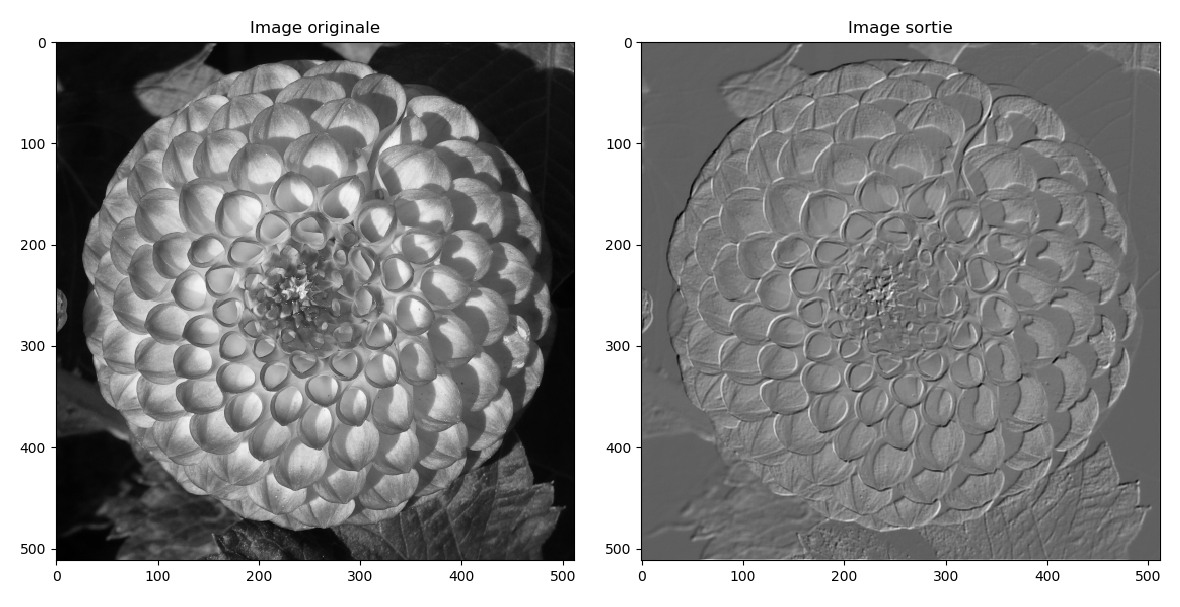
\includegraphics[scale=\myscale,scale=0.3]{figures/ecran-convolution-1}
\end{center}


\begin{lstlisting}
import numpy as np
import matplotlib.pyplot as plt

# Partie A - Importer une image comme un tableau
import imageio
A = imageio.imread('image_avant.png')

# Partie B - Motif de convolution
M = np.array([[-2,-1,0],[-1,1,1],[0,1,2]])

# Partie C - Calcul de la convolution
from scipy import signal
B = signal.convolve2d(A, M, boundary='fill', mode='same')

# Partie D - Affichage des images avant/après
fig = plt.figure(figsize = (10,5))

ax = plt.subplot(1,2,1)
ax.set_title("Image originale")
ax.imshow(A, cmap='gray')

bx = plt.subplot(1,2,2)
bx.set_title("Image sortie")
bx.imshow(B, cmap='gray')

plt.show()

# Partie E - Sauvegarde de l'image
B = np.clip(B,0,255)    # limite les valeurs entre 0 et 255
B = B.astype(np.uint8)  # conversion en entiers
imageio.imwrite('image_apres.png', B)
\end{lstlisting}

Explications.
\begin{itemize}
  \item On utilise le module \ci{imageio} (qui n'est pas installé par défaut) et permet de transformer une image en un tableau \numpy{} (\ci{imread()}) ou l'opération inverse (\ci{imwrite()}).
  \item On prend soin de rendre les coefficients de la matrice $B$ entiers entre $0$ et $255$.
  \item Il existe de multiples variantes du format d'image \og{}.png\fg{}, aussi vos images peuvent s'afficher différemment selon votre visionneuse d'images !
\end{itemize}


On renvoie au chapitre \og{}Convolution\fg{} pour d'autres exemples de motifs intéressants.


%%%%%%%%%%%%%%%%%%%%%%%%%%%%%%%%%%%%%%%%%%%%%%%%%%%%%%%%%%%%%%%%%%%%%
\section{Convolution : une dimension}

%--------------------------------------------------------------------
\subsection{Convolution et vecteurs}

\index{convolution!dimension 1}


Le module \numpy{} permet la convolution de vecteurs.

\begin{lstlisting}
f = np.array([1,0,3,5,1])
g = np.array([1,2,3])  
h = np.convolve(f,g,'same')
\end{lstlisting}

$$f \conv g  = (1, 0, 3, 5, 1) \conv  (1, 2, 3) =  (2, 6, 11, 20, 17).$$

La convolution étendue $f \fullconv g$ s'obtient à l'aide du paramètre \ci{'full'}.
On renvoie à la dernière section du chapitre \og{}Convolution : une dimension\fg{} :
\mycenterline{\ci{
h = np.convolve(f,g,'full')
}}
donne :
$$h = f \fullconv g  = (1, 0, 3, 5, 1) \fullconv  (1, 2, 3) =  (1, 2, 6, 11, 20, 17, 3).$$



%--------------------------------------------------------------------
\subsection{Visualisation}

La visualisation permet de mieux comprendre la convolution en une dimension.
Ici un vecteur $f$ est obtenu en ajoutant un bruit aléatoire à une sinusoïde.
Le vecteur $g$ est un motif qui effectue une moyenne mobile (ici de taille $5$).
La convolution $h = f \conv g$ correspond à un lissage du tracé de $f$.

\begin{center}
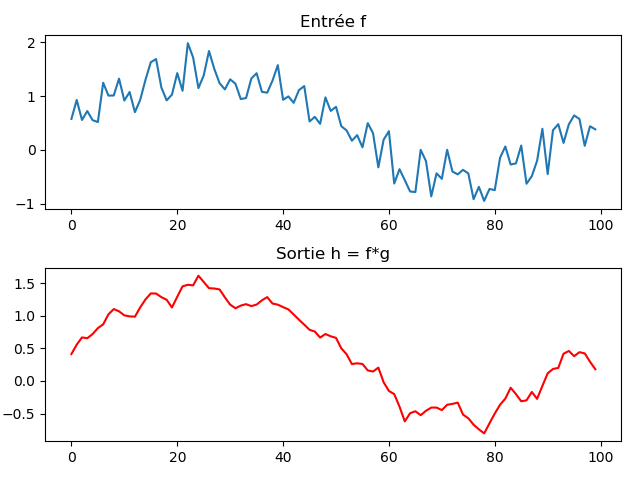
\includegraphics[scale=\myscale,scale=0.7]{figures/pythonconv-1d}
\end{center}

\begin{lstlisting}
N = 100
f = np.sin(np.linspace(0,2*np.pi,N)) + np.random.random(N)
g = 1/5*np.array([1,1,1,1,1])

h = np.convolve(f,g,'same')

ax = plt.subplot(2,1,1)
ax.set_title("Entrée f")
plt.plot(f)

ax = plt.subplot(2,1,2)
ax.set_title("Sortie h = f*g")
plt.plot(h,color='red')

plt.show()
\end{lstlisting}

%--------------------------------------------------------------------
\subsection{Convolution et polynômes}

La convolution est une opération que vous pratiquez déjà sans le savoir !
Si on code un polynôme 
$$P(X) = a_nX^n+a_{n-1}X^{n-1} + a_1X+a_0$$
par la liste de ses coefficients :
$$[P] = (a_n,a_{n-1},\ldots,a_1,a_0),$$
alors la multiplication $P \times Q$ de deux polynômes correspond au produit de convolution des listes des coefficients :
$$[P\times Q] = [P] \fullconv [Q].$$

Par exemple, pour 
$$P = X^3 + 2X^2 +3X + 4 \qquad [P] = (1,2,3,4)$$
et
$$Q = 5X^2 + 6X +7 \qquad [Q] = (5,6,7),$$
on calcule la convolution étendue des coefficients :
$$[P] \fullconv [Q] = (1,2,3,4) \fullconv (5,6,7)
= (5, 16, 34, 52, 45, 28).$$
Cela correspond aux coefficients de $P \times Q$ :
$$P \times Q = 5X^5 + 16X^4 + 34X^3 + 52X^2 + 45X + 28.$$


%--------------------------------------------------------------------
\subsection{Traitement du signal}

\begin{center}
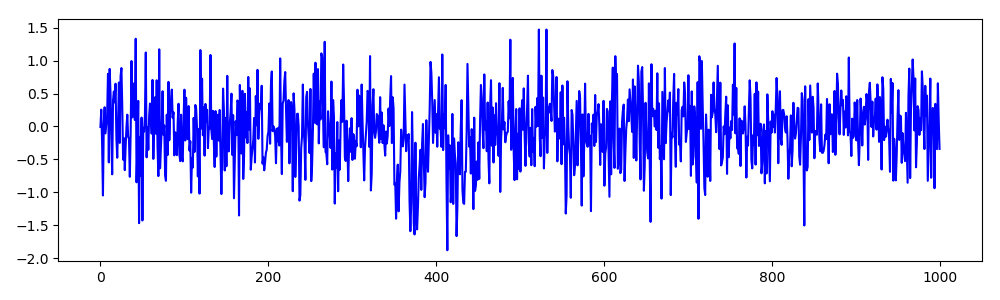
\includegraphics[scale=\myscale,scale=0.5]{figures/correlation1d-3}

\textbf{Signal reçu par un radar : où est l'avion ?}
\end{center}



\textbf{Radar.}
Nous avons vu que la convolution permet le traitement d'un signal : lissage d'une courbe (voir ci-dessus), mais aussi d'autres opérations (voir le chapitre \og{}Convolution : une dimension\fg{}).
Une autre application est la détection radar.
En voici le principe : le radar émet un signal, les ondes atteignent un objet (un avion par exemple) et sont renvoyées par réflexion, le radar reçoit ce signal réfléchi. Le temps mis par les ondes pour effectuer l'aller-retour permet de calculer la distance à l'objet.


\myfigure{0.7}{
\tikzinput{fig-radar}
}


Dans la pratique c'est plus compliqué : le signal émis est bien connu, mais le signal reçu est composé de l'onde réfléchie à laquelle se superpose un bruit aléatoire lié à l'environnement (les nuages, les oiseaux\ldots).


\begin{center}
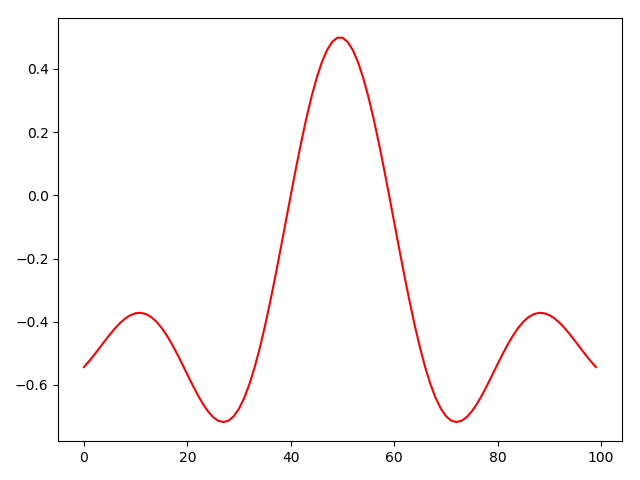
\includegraphics[scale=\myscale,scale=0.4]{figures/correlation1d-1}

\textbf{Impulsion $g$ émise par le radar.}
\end{center}

\begin{center}
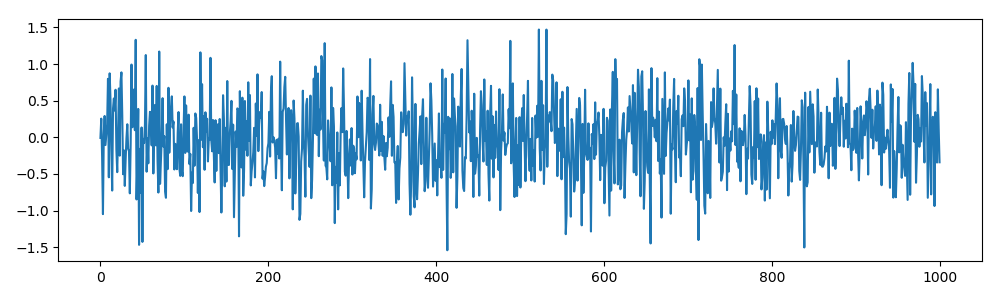
\includegraphics[scale=\myscale,scale=0.5]{figures/correlation1d-2}

\textbf{Bruit.}
\end{center}

\begin{center}
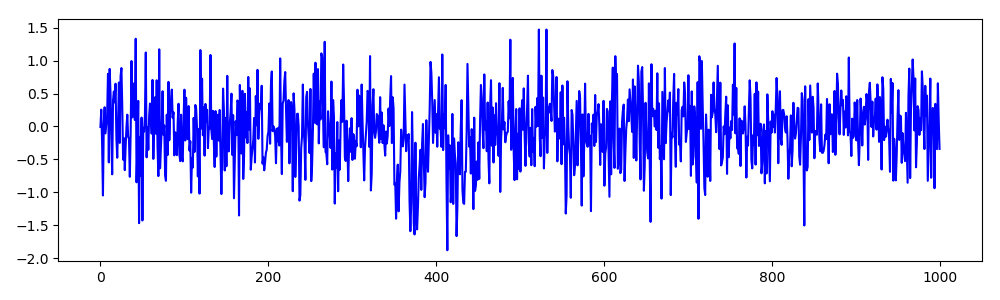
\includegraphics[scale=\myscale,scale=0.5]{figures/correlation1d-3}

\textbf{Signal $f$ reçu par le radar}
\end{center}

Sur l'exemple ci-dessus, le signal $f$ est obtenu comme la somme d'un bruit (un signal aléatoire) et une copie de l'impulsion $g$ entre les abscisses $350$ et $450$. Regardez bien la différence entre le bruit et le signal $f$ autour de l'abscisse $400$ !

Comment retrouver la position de l'impulsion $g$ à partir du signal reçu $f$ ?

\bigskip
\textbf{Corrélation.}

Nous n'allons pas utiliser la convolution, mais la \defi{corrélation}\index{convolution!correlation@corrélation} qui est une opération similaire sauf que le motif n'est pas renversé.
\myfigure{0.7}{
\tikzinput{fig-correlation1d}
}

Par exemple si $f =  (1, 0, 3, 5, 1)$ et $g = (1, 2, 3)$ alors la corrélation de $f$ avec $g$ vaut $h = (2, 10, 21, 16,  7)$.

\bigskip
\textbf{Détection.}

On note $g$ le signal émis par le radar, c'est un vecteur (ici de longueur $100$).
On note $f$ le signal reçu par le radar, c'est un vecteur (ici de longueur $1000$).
On calcule la corrélation $h$  de $f$ avec $g$, c'est un vecteur (ici de longueur $1000$).

\begin{center}
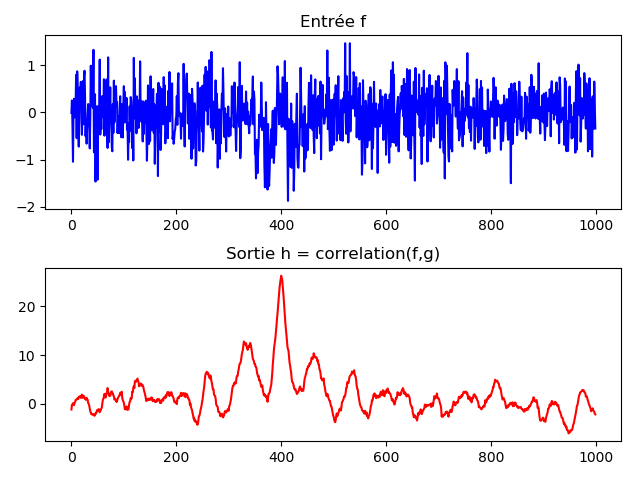
\includegraphics[scale=\myscale,scale=0.7]{figures/correlation1d-4}
\end{center}

Le pic observé correspond au signal renvoyé par l'avion. Sur l'exemple, ce signal est détecté en position $400$ ($400$ millisecondes par exemple). Ce qui permet de calculer la distance du radar à l'avion. Plusieurs mesures permettraient même de déterminer sa vitesse.
% Noter que dans le vecteur $h$, calculé par corrélation, on ne retrouve pas l'impulsion originelle $g$ émise par le radar. La corrélation permet de détecter la présence de l'impulsion $g$ et sa position.

%%%%%%%%%%%%%%%%%%%%%%%%%%%%%%%%%%%%%%%%%%%%%%%%%%%%%%%%%%%%%%%%%%%%%
\section{Corrélation en deux dimensions}

\index{convolution!dimension 2}

Sur cette photo vous reconnaissez immédiatement un chat ! 
\begin{center}
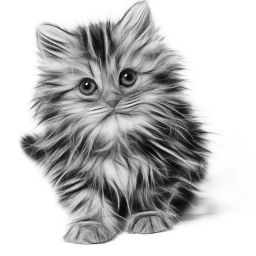
\includegraphics[scale=\myscale,scale=0.5]{figures/chat}
\end{center}
Mais pour un ordinateur ce n'est qu'un amas de pixels plus ou moins gris.

Ci-dessous, voici une autre image qui montre mieux ce que peut représenter une image pour 
un ordinateur. Que voyez-vous sur cette image : un chat, un chien ou un bonhomme qui sourit ?

\begin{center}
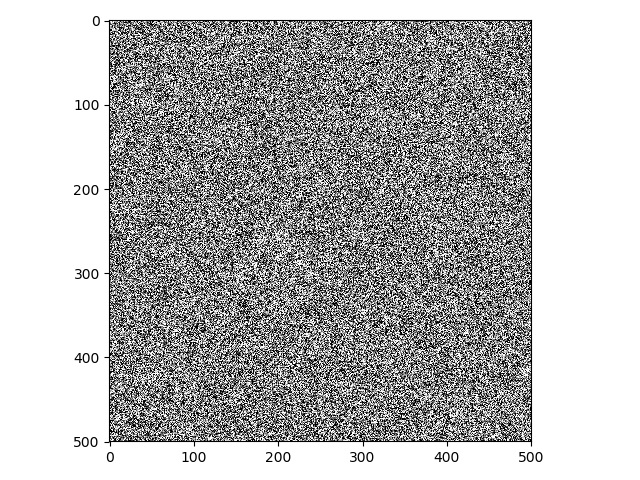
\includegraphics[scale=\myscale,scale=0.5]{figures/correlation2d-3}
\end{center}


Nous allons voir que la convolution permet de retrouver un motif dans une image, exactement comme on l'a fait avec le radar dans le cas d'une dimension.
Voici le motif qu'il fallait \og{}voir\fg{} dans l'image ci-dessus.
\begin{center}
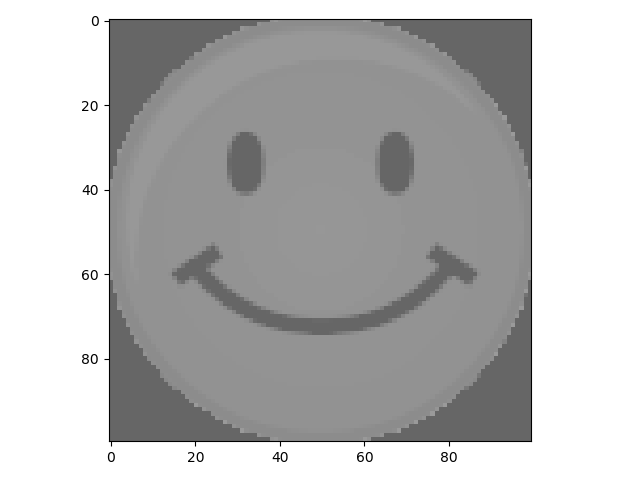
\includegraphics[scale=\myscale,scale=0.3]{figures/correlation2d-1}
\end{center}

Tout d'abord, quelques informations pour obtenir une image brouillée. On part d'une image $500\times 500$ de pixels (ici en niveaux de gris) aléatoires (image de gauche ci-dessous). On superpose le motif \og{}smiley\fg{} de taille $100 \times 100$ à une partie de cette l'image. On obtient donc une image avec un motif caché (image de droite ci-dessous).

%\begin{minipage}{0.49\textwidth}
%\begin{center}
%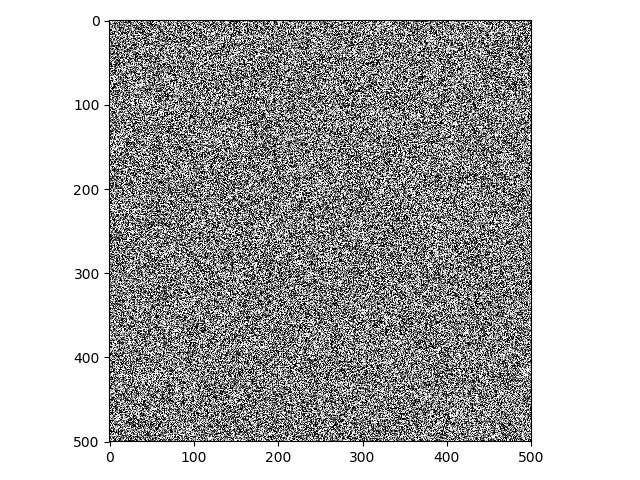
\includegraphics[scale=\myscale,scale=0.5]{figures/correlation2d-2}
% 
%\textbf{Image crée par des pixels aléatoires}  
% 
%\end{center}
%\end{minipage}
%\begin{minipage}{0.49\textwidth}
%\begin{center}
% 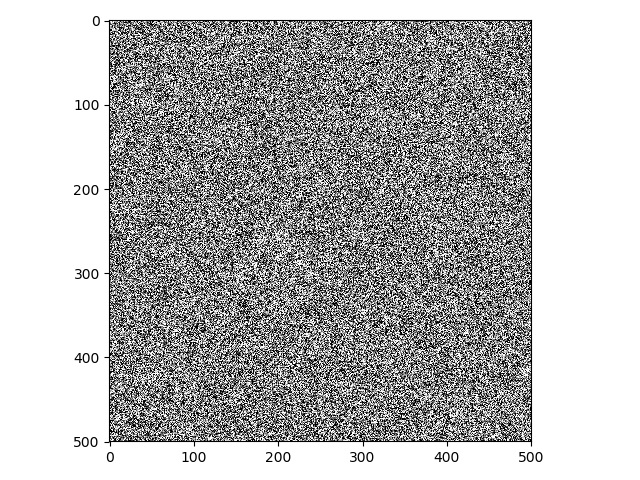
\includegraphics[scale=\myscale,scale=0.5]{figures/correlation2d-3}
%
%  \textbf{Image avec le motif incrusté}  
%\end{center} 
%\end{minipage}


\hspace*{-2em}
\begin{minipage}{\textwidth}
\myfigure{1}{
\tikzinput{fig-correlation2d}
}
\end{minipage}



On calcule la corrélation entre l'image et le motif.
La corrélation en deux dimensions, c'est comme la convolution mais sans retourner la matrice du motif.
La corrélation indique si le motif est présent ou pas dans l'image et si oui, à quel endroit.

\begin{center}
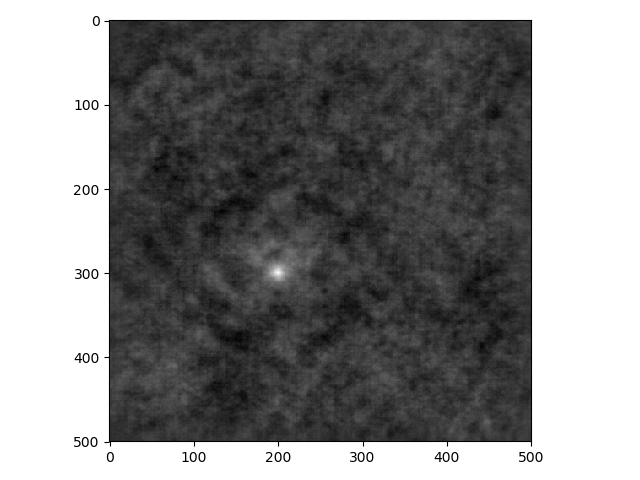
\includegraphics[scale=\myscale,scale=0.45]{figures/correlation2d-4}
\end{center}
Sur notre exemple la corrélation indique une correspondance autour du point $(200,300)$.

\end{document}
